\documentclass[11 pt, twocolumn]{article}

\usepackage{hyperref}
\usepackage{titling}
\usepackage{amsmath}
\usepackage{algorithm}
\usepackage[noend]{algpseudocode}
\usepackage[margin=1in]{geometry}
\usepackage{graphicx}
\usepackage{color}

\makeatletter
\def\BState{\State\hskip-\ALG@thistlm}
\makeatother

\setlength{\droptitle}{-5em}
 
\title{When AI Gets Bored}
\author{Nevo Agmon 203116769, Yuval Shildan 205799307}
\date{Winter 2019}

\newcommand{\todo}[1]{}
\renewcommand{\todo}[1]{{\color{red} TODO: {#1}}}

\begin{document}
\maketitle
\section{Abstract}
In the field of AI Reinforcement Learning (RL) is used to solve problems requiring an agents to interact with a given environment. Specifically, Q - Learning is a model free algorithm with the goal of learning a policy which tells the agent what action to take in a given state.

Evolution Strategies (ES) is a family of algorithms based of the idea of natural evolution that have recently shown to be comparable to the state of the art in Q - Learning on a challenging set of problems. Having the benefit of being highly parallelizable, thus reducing training duration from several days to a matter of hours.

\todo{need to change this, we dont use RL} ES and RL have different learning characteristics, resulting in different strengths and weaknesses. In this paper we describe a very simple canonical ES algorithm, and try to improve it's performance with ideas from more traditional RL in order to show that the combination of both could possibly advance upon the current state of the art.


\section{Problem Description}
Our work is based on the paper \emph{Back to Basics: Benchmarking Canonical Evolution Strategies for  Playing Atari}, by Chrabaszcz et al. \cite{canonical} in which described a canonical ES algorithm and is benchmarked on a series of atari games. The algorithm is described in Algorithm \ref{alg_canonical}.

\subsection{CanonicalES}
As can be seen the algorithm is based on an iterative process where at every iteration $t$ we create a set of $\lambda$ offspring. This is done by adding a mutation to the base policy, the mutation is given by the mutation step size multiplied by a sampled random noise. After offspring creation we evaluate each offspring's policy on the environment. Once this process in done, we choose the $mu$ best performing offspring and update the base policy with the weighted sum of their mutation.

This algorithm is relatively simple, and as mentioned before is loosely based on the idea of natural evolution. Meaning, offspring are passed the "genetic material" from their parent with a random mutation, evolution occurs when processes like natural selection acts on these variations and results in some characteristics being more prominent in the population while others become sparse.

\begin{algorithm}
\scriptsize
\caption{Canonical ES Algorithm}\label{alg_canonical}
\hspace*{\algorithmicindent} \textbf{Input:} \\
\hspace*{\algorithmicindent} $\sigma$ - Mutation step size\\
\hspace*{\algorithmicindent} $\theta_0$ - Initial Policy parameters\\
\hspace*{\algorithmicindent} $F$ - Policy evaluation function\\
\hspace*{\algorithmicindent} $\lambda$ - Offspring population size\\
\hspace*{\algorithmicindent} $\mu$ - Parent population size\\
\hspace*{\algorithmicindent} \textbf{Initialize:}
\begin{align*}
  &w_i=\frac{\log{(\mu + 0.5)}-\log{(i)}}{\sum_{j=1}^{\mu} \log{(\mu + 0.5)}-\log{(j)}}&
\end{align*}
\begin{algorithmic}[1]
      \For{$t \in \{0,1,\dots\}$}
      	\For{$i \in \{1,\dots,\lambda\}$}
      	\State Sample noise: $\epsilon_i \sim \mathcal{N}(0,I)$
      	\State Evaluate score in the game: $s_i \gets F(\theta_t+\sigma*\epsilon_i)$
      	\EndFor
      	\State Sort($\epsilon_1,\dots,\epsilon_\lambda$) according to $s$ ($\epsilon_i$ with best $s_i$ first)
      	\State Update policy: $\theta_{t+1} \gets \theta_t + \sigma * \sum_{j=1}^{\mu} w_j*\epsilon_j$
      	\State Optionally update step size $\sigma$
      \EndFor
\end{algorithmic}
\end{algorithm}

\subsection{Main Objective}
This approach yielded good results in a short period of training, as shown by Chrabaszcz et al. but has few drawbacks, as shown in figure \ref{fig:canonical_results}. Mainly the policy tends to reach some local optima and plateau. This leads to our main objective for this paper, define a set of improvements to encourage the policy to seek for a better solution and reduce the tendency to plateau. To accomplish this objective we look at the work done by Conti et al. \cite{improveES} in the paper \emph{Improving Exploration in Evolution Strategies for Deep Reinforcement Learning via a Population of Novelty-Seeking Agents}. In their paper Conti et al. tries to optimize an ES algorithm (related but not the same and Chrabaszcz et al.'s canonical one) to seeking for novel decisions to address the very same problem.

\begin{figure}[h!]
  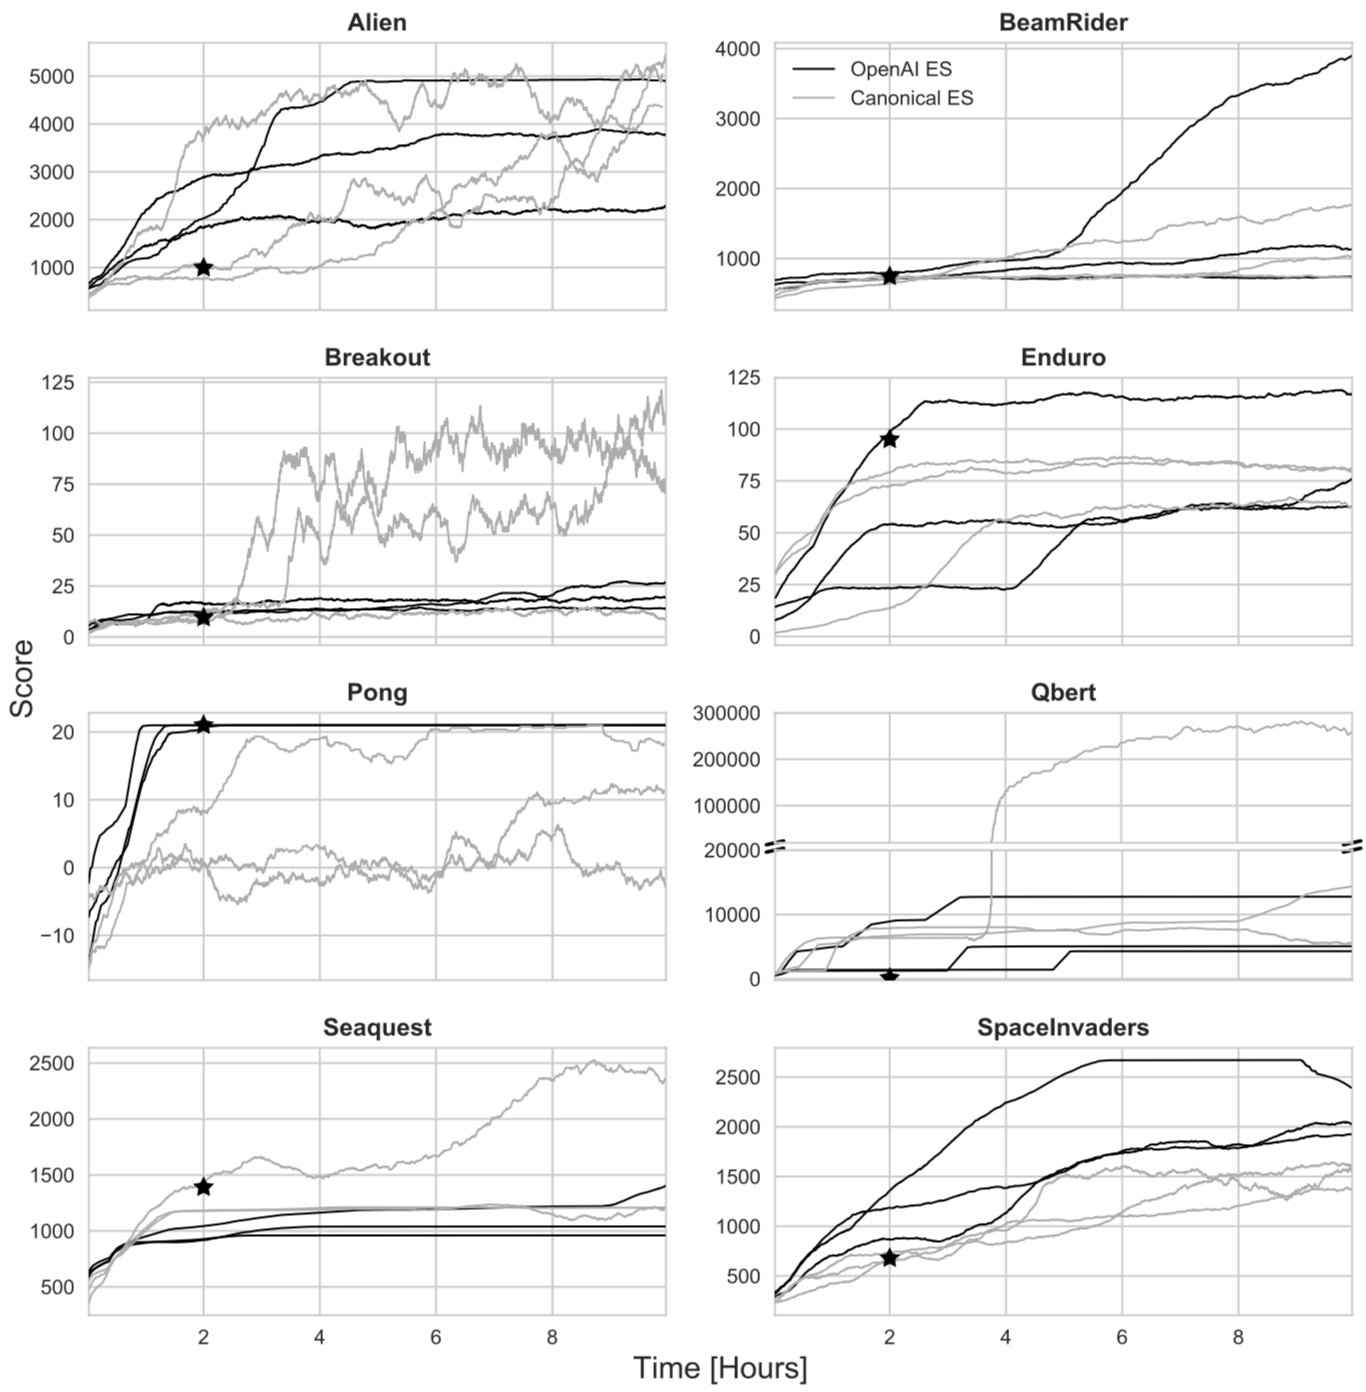
\includegraphics[width=\linewidth]{canonical_train_res.png}
  \caption{Training curves for Chrabaszcz et al.'s CanonicalES algorithm. The algorithm often reach local optima and plateau. \todo{change image, remove OpenAI from graph}}
  \label{fig:canonical_results}
\end{figure}

\section{Method Description}
To define a set of improvements to try and rectify the described problem we first had to make an assumption as to what causes this behavior. Our assumption was that because the algorithm optimizes for immediate reward, it can miss on the opportunity for better performance and greater overall reward. Meaning, we want to optimize for overall game performance, preferably averaging performance over multiple runs. Unfortunately, since a single game is comprised of a large number of decisions, if we track the end game result and optimize accordingly we could not tell what is the state and action relations that improve performance and therefore optimize poorly.

Therefore, we decided to focus on two aspects of the algorithm for improvement:
\begin{enumerate}
	\item Searching for new untried moves.
	\item Reproduce population from multiple samples.
\end{enumerate}

\subsection{Novelty Search}
In order to reduce the tendency to reach local optima biased by short term reward we introduce Novelty Search (NS). As shown by Conti et al. NS encourages the policy to act differently than previous seen behavior. To encourage different behaviors the algorithm uses a \emph{novelty} value computed for each policy to represent the amount of innovation of the current policy with respect to the previously seen policies.

Formally, given a parameter vector $\theta$  and policy $\pi_\theta$ we define a \emph{behavior} mapping $b(\pi_\theta)$, this can be thought of as an embedding of the policy output to a vectorized form. We then save these behavior representations in a set $A$ and evaluate the \emph{novelty} of the current policy as the average distance between it and the $k$ nearest neighbors from the saved set $A$.

\begin{align*}
N(\theta, A)=N(b(\pi_\theta),A)&=\frac{1}{|A|}\sum_{j\in A} \|b(\pi_\theta)-b(\pi_j)\|_2\\
S=kNN(b(\pi_\theta),A)&=\{b(\pi_1),b(\pi_2), \dots,b(\pi_k)\}
\end{align*}

Now, instead of choosing the meta population based on the policy's reward we want to take into account both the reward and policy's novelty. We assign each policy a performance score $\hat{s}$, it's novelty value added to it's reward:

\begin{equation*}
\hat{s}=N(\pi_\theta,A)+F(\theta)
\end{equation*}

To update the policy we can add the reward and novelty values to the update step thus encouraging the policy to move in the direction where the gradients of novelty and reward are greater. as a first try we add the novelty and reward average:

\begin{equation*}
\theta_{t+1}\gets\theta_t+\sigma*\sum_{j=1}^{\mu}w_j*\epsilon_j*\frac{N(\theta_t^j,A)+F(\theta_t^j)}{2}
\end{equation*}

To further improve our optimization we can weight the novelty and reward values according to the state we are in, as opposed to always having their average.

\begin{equation*}
\theta_{t+1}\gets\theta_t+\sigma*\sum_{j=1}^{\mu}w_j*\epsilon_j*(1-\hat{w})N(\theta_t^j,A)+\hat{w}F(\theta_t^j)
\end{equation*}

Starting with only optimization for reward ($\hat{w}=1$), we can track the policy's performance, if we improve our game we want to optimize for reward so in every iteration we increase the weight. If on the other hand we stop improving, it means we got into a plateau, we will start decreasing the weight so that we will optimize for novelty.

\subsection{Population Reproduction}
The CanincalES algorithm, as described, takes a meta population of size $mu$ of best performing offspring and uses the weighted sum of their mutation as the learned parameter, updating the base policy with that weighted mutation. This may seem like a good idea, take the best of the population and reproduce them. But, if we take natural evolution as our guide for building our algorithm, then we know that the fact a beneficial mutation occurred is not directly correlated the offspring's ability to reproduce. Rather it simply increases the odes for the offspring reproduction and keep the mutation in the population. Therefore, instead of taking the best set of offspring we give each offspring a probability score based on it's performance and sample the set from the population according to the said probability.

We would like to use the performance score $\hat{s}$ we defined above to compute the probability \todo{explain about normalization and sampling}

\subsection{Implementation}
\todo{pca and knn distance then the final algorithm}

\section{Results}
\section{Conclusion}

\bibliography{when_AI_Gets_Bored} 
\bibliographystyle{ieeetr}
\end{document}